% LTeX: language=de-CH

\chapter{Ein eigener Zugang -- methodisch und angewandt} \label{sec:methodik}

In diesem Kapitel positioniere ich den methodischen Zugang meiner Arbeit im Kontext bestehender Ansätze zur Erhebung situativer Daten. Zunächst ordne ich die verwendete Erhebungslogik begrifflich ein und grenze sie gegenüber verwandten Verfahren ab. Danach stelle ich bestehende digitale Erhebungsplattformen vor, die ähnliche Zielsetzungen verfolgen. Die vergleichende Analyse zeigt Gemeinsamkeiten, Unterschiede und Leerstellen auf und dient als Grundlage, um meine eigene Herangehensweise präzise zu positionieren.

Die konkreten technischen und inhaltlichen Umsetzungen -- etwa die Entwicklung der App \gls[noindex]{intermind} (\cref{sec:entwicklung_app}) oder die Gestaltung des Fragebogens (\cref{sec:fragebogenentwicklung}) -- erläutere ich in den folgenden Kapiteln ausführlich.


\section{Situationen erfassen -- Wiederholte Befragung mit ESM, EMA und GEMA}

Die systematische Erhebung von situiertem Wohlbefinden erfordert Methoden, die subjektive Erfahrungen möglichst unmittelbar und kontextspezifisch erfassen. Retrospektive Selbstauskünfte sind hierfür nur begrenzt geeignet, da sie Verzerrungen durch selektive Erinnerung oder nachträgliche Neubewertung unterliegen \parencite[\textit{Recall Bias} \gls{vgl},][]{kahnemanDevelopmentsMeasurementSubjective2006}. Um solche Verzerrungen zu vermeiden, wurde bereits in den 1980er-Jahren die \emph{\glsxtrfull{esm}}-Methode entwickelt. Dieses Verfahren basiert auf der mehrfach wiederholten Erhebung subjektiver Zustände im Alltag -- etwa durch zeitlich zufällig verteilte Aufforderungen an Teilnehmende, ihre momentane Stimmung oder Tätigkeit zu protokollieren \parencite{csikszentmihalyiValidityReliabilityExperienceSampling1987}. Ziel ist es, das Erleben möglichst nah am Zeitpunkt der Erfahrung und im Kontext zu erfassen. Typisch für \glsxtrshort{esm} sind kurze, wiederholte Abfragen zu spezifischen psychologischen Konstrukten, die Verzerrungen minimieren und einen Einblick in die dynamischen Prozesse individuellen Erlebens erlauben.

Während \glsxtrshort[noindex]{esm} ursprünglich primär als psychologisches Messinstrument konzipiert wurde, wurde der Ansatz in den 1990er-Jahren durch die \emph{\glsxtrfull{ema}}-Methode\footnotemark methodologisch erweitert. Mit der \glsxtrshort{ema}-Methode lassen sich zusätzlich explizit physiologische, verhaltensbezogene und weitere kontextuelle Daten erfassen \parencite{shiffmanEcologicalMomentaryAssessment2008}. \glsxtrshort{ema} erlaubt dadurch eine umfassendere Erfassung individueller Zustände und deren Kontextbedingungen. Im Gegensatz zu \glsxtrshort[noindex]{esm} ist \glsxtrshort{ema} zudem methodologisch offener für die Integration verschiedenster Datenquellen und Analyseebenen.

\footnotetext{Der Begriff \textit{ecological} verweist hierbei nicht auf \enquote{natürliche} Umgebungen, sondern auf die Wechselbeziehungen zwischen Lebewesen und ihrer jeweiligen Umwelt -- unabhängig davon, ob diese natürlich, sozial oder technisch geprägt ist.}

Mit der zunehmenden Verbreitung von \gls{gps}-fähigen Endgeräten wurde \glsxtrshort[noindex]{ema} in den 2010er-Jahren durch das Konzept der \emph{\glsxtrfull{gema}}-Methode ergänzt. \glsxtrshort{gema} kombiniert subjektive Momentaufnahmen mit objektiven, räumlich verortbaren Kontextinformationen wie Standort, Wetterbedingungen, Lärmpegel oder Bebauungsstruktur \parencite{kirchnerSpatiotemporalDeterminantsMental2016}. Im Unterschied zu \glsxtrshort{ema} legt \glsxtrshort{gema} damit besonderen Wert auf die räumliche Kontextualisierung der erhobenen Daten. Dabei werden subjektive Erfahrungen nicht nur als zeitlich-situativ, sondern explizit als räumlich-situiert betrachtet. Entscheidend ist hierbei die Möglichkeit, emotionales Erleben in direkten Bezug zum spezifischen räumlich-materiellen Kontext zu setzen und dadurch differenzierte Aussagen über räumliche Einflüsse auf das Erleben zu ermöglichen. \glsxtrshort{gema} erlaubt dadurch eine komplexere Analyse der Wechselwirkungen zwischen individuellen Erfahrungen und räumlicher Umgebung und öffnet die methodologische Perspektive für interdisziplinäre, insbesondere geographische Fragestellungen.

Tatsächlich greifen viele \gls{gema}-Studien geographische Fragestellungen auf, auch wenn sie häufig in gesundheitlichen Forschungskontexten erscheinen. So verknüpfen \textcite{gasikUsingGeographicMomentary2025} Echtzeitangaben zu Sicherheitsempfinden, Stress und Stimmung von Menschen mit \gls{hiv} in New Orleans mit räumlichen Indikatoren wie Gewaltdichte, Alkoholverkaufsstellen oder Brachflächen. \textcite{zhangGeographicEcologicalMomentary2020} untersuchen, wie situative Lärmbelästigung an unterschiedlichen Aufenthaltsorten in Abhängigkeit vom Aktivitätskontext und der täglichen akustischen Belastung wahrgenommen wird. \textcite{zhangTemporalityGeographicContexts2023} analysieren die Wirkung von Umweltfaktoren auf die Stimmung nicht nur in Echtzeit, sondern auch kumulativ und zeitverzögert.

\section{Anknüpfen und Abgrenzen -- Vergleich mit bestehenden Instrumenten}
\label{sec:vergleich_bestehender_instrumente}

Die im Rahmen dieser Arbeit entwickelte App \gls[noindex]{intermind} bewegt sich im Spannungsfeld zweier methodischer Herangehensweisen: der Echtzeiterhebung räumlich kontextualisiertem (Un\nobreakdash-)Wohlbefinden (wie bei \gls[noindex]{urbanmind}) und der explizit intersektionalen Analyse subjektiver Raumwahrnehmungen (wie bei \textit{\gls[noindex]{reliefmaps}}). Beide bestehenden Instrumente bilden zentrale Referenzpunkte für die Konzeption des eigenen Ansatzes, da sie jeweils zentrale Teilaspekte adressieren: Während \gls[noindex]{urbanmind} eine räumlich verortete Echtzeiterhebung subjektiven Wohlbefindens umsetzt, fokussiert \textit{\gls[noindex]{reliefmaps}} auf eine reflexive, intersektionale Kartierung räumlicher Erfahrung.

Die Auswahl dieser beiden Erhebungsplattformen erfolgte zum einen aufgrund ihrer inhaltlichen Nähe zum eigenen Untersuchungsinteresse, zum anderen auch aus praktischer Zugänglichkeit: Aktuell ist \gls{urbanmind} eines der wenigen öffentlich zugänglichen \glsxtrshort{gema}-Tools, das in wissenschaftlichen Studien eingesetzt wird.\footnote{Die Dokumentation einer ähnlichen Plattform \textit{\glsxtrfull[noindex]{health}} \parencite{wrayHealthyEnvironmentsActive2025} wurde während der Entstehung dieser Arbeit als Preprint veröffentlicht.} \textit{\gls[noindex]{reliefmaps}} wiederum ist der einzige bekannte Ansatz, der intersektionale Raumwahrnehmungen systematisch operationalisiert und ist durch seine Kombination aus Emotionalität, Raumbezug und \glspl{identitaetsachse} besonders anschlussfähig für das vorliegende Projekt.

Der folgende Vergleich dient dazu, methodische Gemeinsamkeiten und Unterschiede herauszuarbeiten und den eigenen methodischen Zugang klar zu positionieren.


\subsection*{\gls[noindex]{urbanmind}: Ein vielseitige, aber nicht quelloffene Plattform}

\gls{urbanmind}\footnote{\href{https://urbanmind.info/}{urbanmind.info}} ist eine Plattform für \glsxtrshort{gema}-Studien: Sie kombiniert standardisierte Echtzeiterhebungen subjektiven Wohlbefindens mit automatisiert erfassten Geodaten und erlaubt so die kontextsensitive Analyse psychischer Gesundheit im Alltag \parencite{bakolisUrbanMindUsing2018}. Die zugrunde liegende Smartphone-App kann flexibel an unterschiedliche Forschungsfragen angepasst werden.

\gls{urbanmind} wird in mehreren Studien eingesetzt, um Zusammenhänge zwischen Umweltfaktoren und psychischer Gesundheit zu analysieren: So zeigen \textcite{bakolisUrbanMindUsing2018}, dass natürliche Elemente wie Himmel, Wasser oder Grünflächen kurzfristig das Wohlbefinden steigern können, \textcite{bergouMentalHealthBenefits2022} belegen vergleichbare Effekte für Aufenthalte an Flüssen und Kanälen, \textcite{hammoudLonelyCrowdInvestigating2021} identifizieren Zusammenhänge zwischen sozialer Dichte, dem Gefühl sozialer Inklusion und situativer Einsamkeit, und \textcite{hammoudSmartphonebasedEcologicalMomentary2022} finden Hinweise darauf, dass Vögel die psychische Verfassung nachhaltig verbessern können.

Während diese Studien wichtige Beiträge zur Analyse kontextueller Einflüsse auf psychische Gesundheit leisten, bleibt eine explizit intersektionale Perspektive bislang unberücksichtigt. Zwar erlaubt die App die Erfassung zentraler demografischer Merkmale, dieses Potenzial wird in den vorliegenden Auswertungen jedoch nicht genutzt -- obwohl entsprechende Analysen innerhalb der bestehenden Infrastruktur prinzipiell möglich wären.


\begin{figure}[h]
    \centering
    \begin{minipage}[t]{0.38\textwidth}
        \centering
        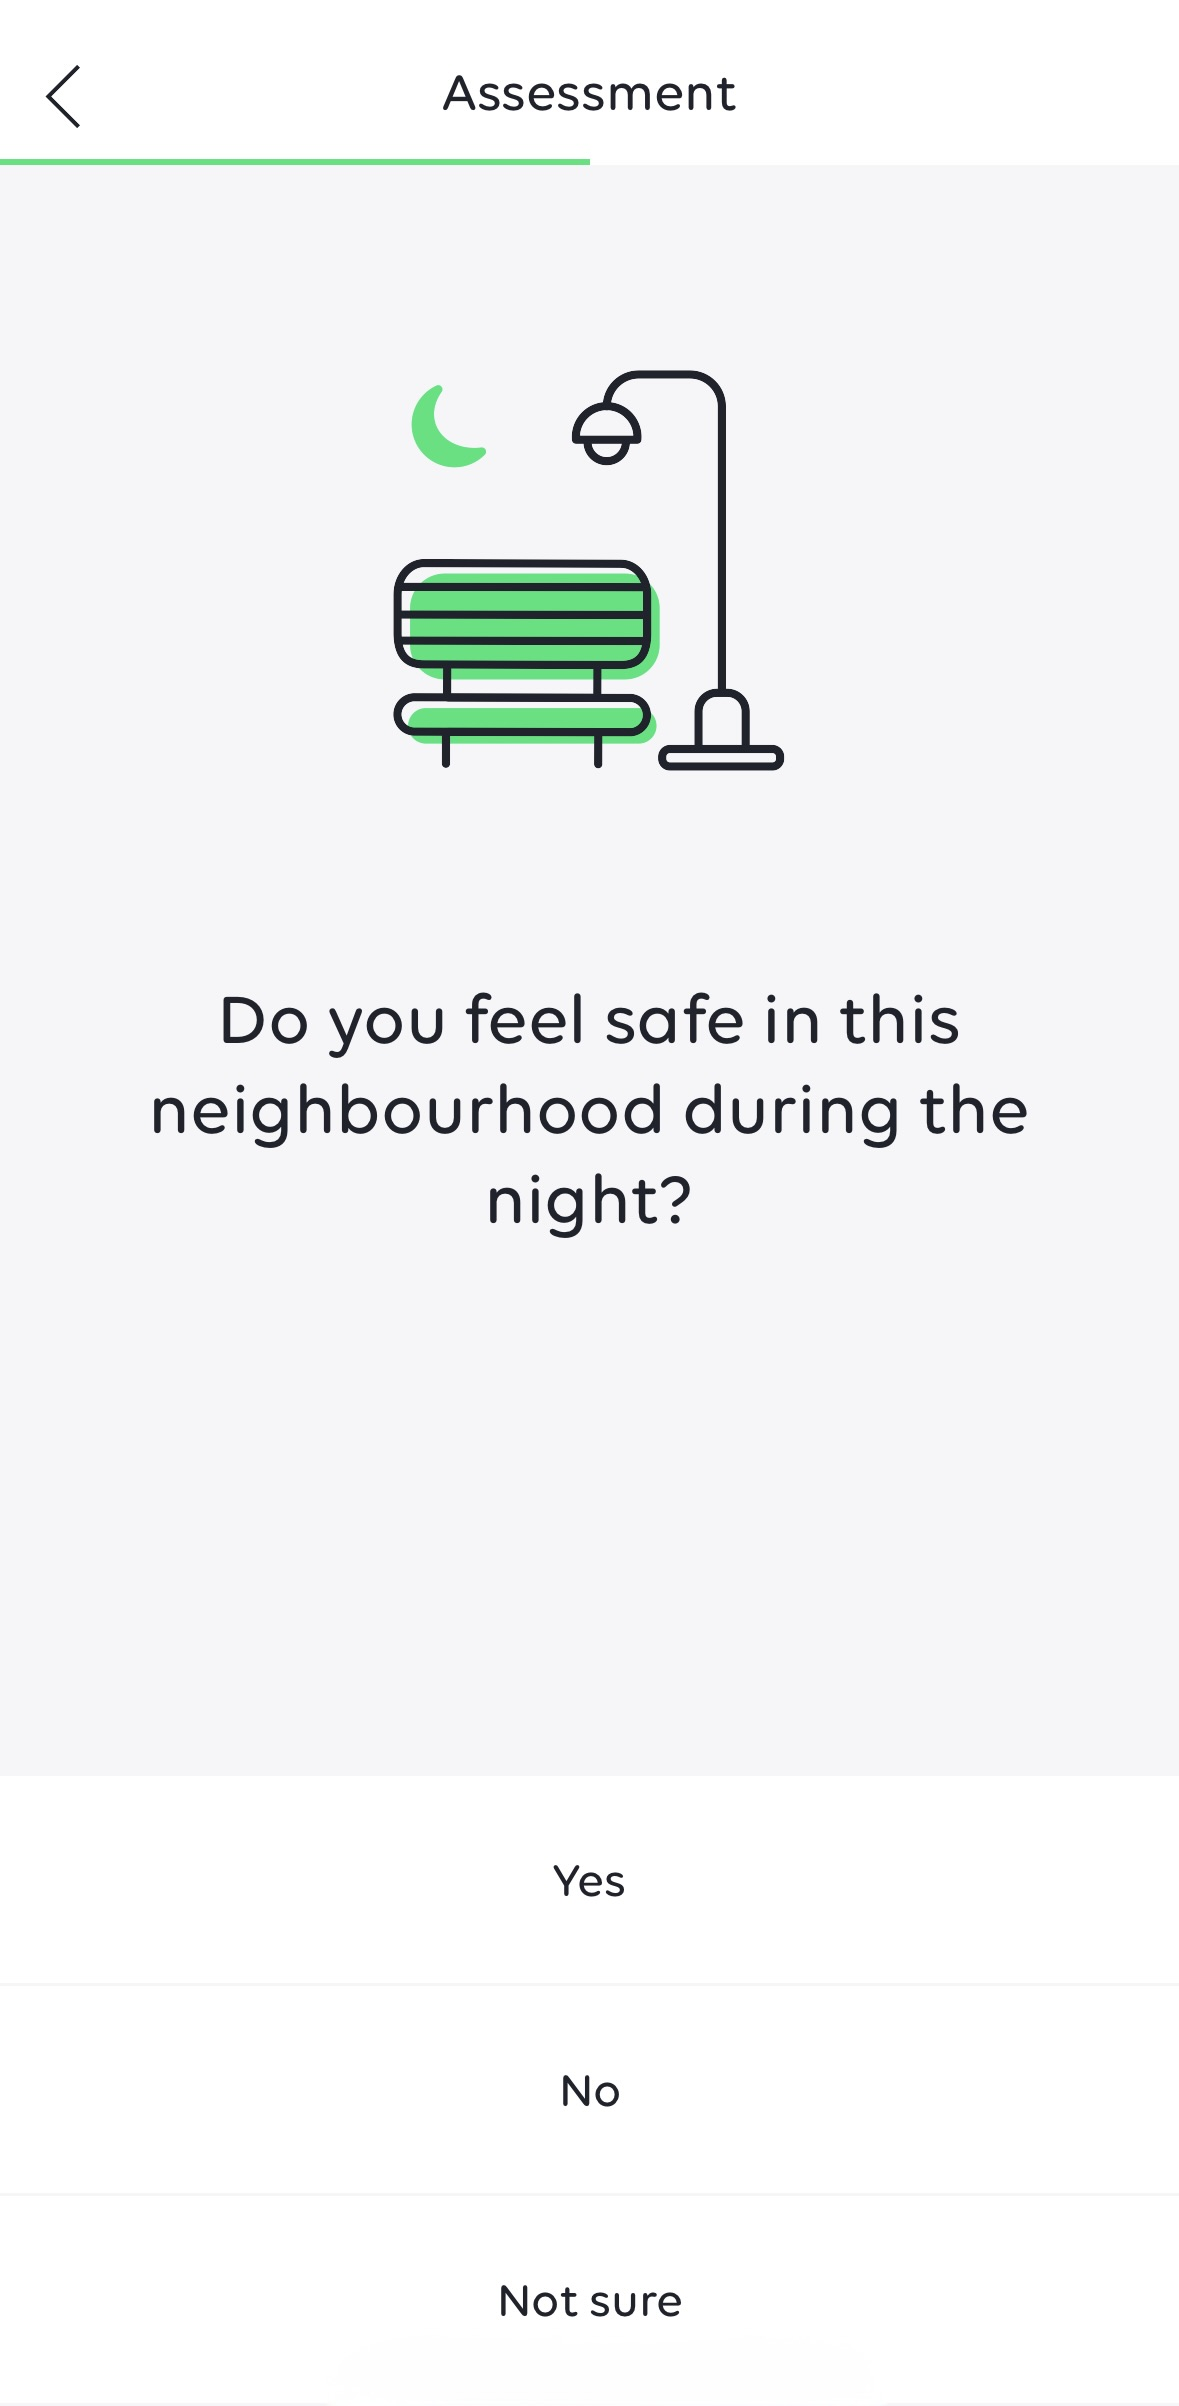
\includegraphics[width=\textwidth]{Arbeit/Bilder/urban_mind01.jpeg}
        \caption{Screenshot einer typischen Frageseite aus der \gls{urbanmind}-App}
        \label{fig:urban_mind_screenshot_1}
    \end{minipage}
    \hspace{0.1\textwidth}
    \begin{minipage}[t]{0.38\textwidth}
        \centering
        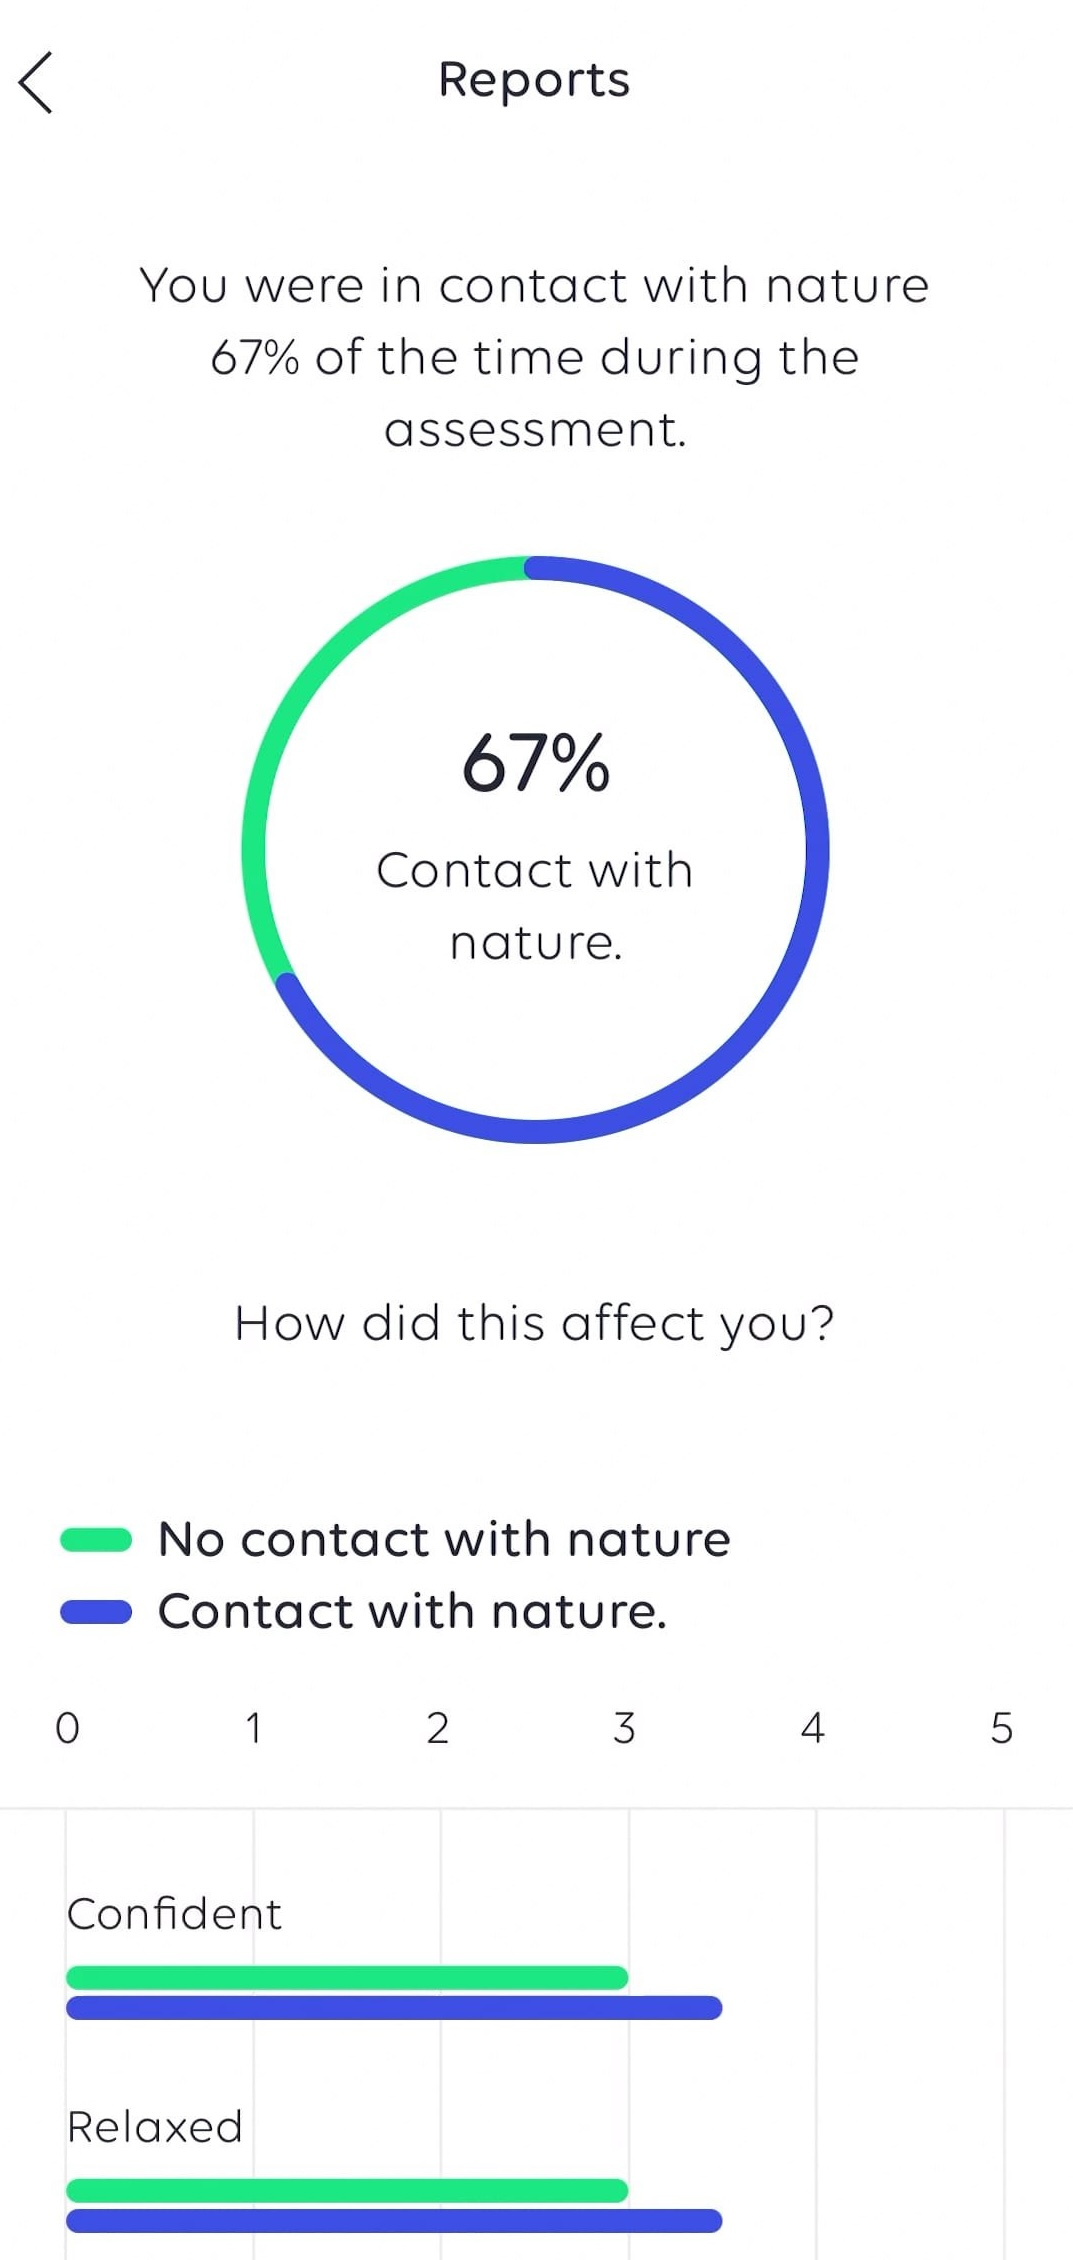
\includegraphics[width=\textwidth]{Arbeit/Bilder/urban_mind_report.jpg}
        \caption{Screenshot eines individuellen Reports aus der \gls{urbanmind}-App}
        \label{fig:urban_mind_report}
    \end{minipage}
\end{figure}

\gls{urbanmind} zeichnet sich durch eine einfache und ansprechend gestaltete Benutzeroberfläche aus, die eine niedrige Einstiegshürde für die Teilnehmenden bietet (siehe \cref{fig:urban_mind_screenshot_1}). Im Mittelpunkt stehen kurze Befragungen, die jeweils etwa drei Minuten dauern und die Teilnehmenden abhängig von der konkreten Studie \gls{bspw} zu ihrem momentanen Wohlbefinden, aktuellen Tätigkeiten sowie ihrer direkten räumlichen und sozialen Umgebung befragen. Diese Befragungen werden in den meisten Studien drei Mal täglich über eine Dauer von zwei Wochen durchgeführt. Teilnehmende werden dazu jeweils mit einer Push-Mittielung benachrichtigt und haben anschliessend jeweils eine Stunde Zeit, um die Befragung abzuschliessen.

Zusätzlich zu den standardisierten Fragebogen-Items erfasst die App kontinuierlich im Hintergrund Standortdaten mittels \gls{gps} sowie optional Gesundheits- und Aktivitätsdaten (\gls{zb} Schrittzahl, zurückgelegte Distanzen), sofern die Teilnehmenden diese Datenerfassung explizit freigeben. Weiter bietet \gls{urbanmind} die Möglichkeit, kurze Audioaufnahmen und Fotos zu teilen. Diese Mediendateien werden nicht nur für wissenschaftliche Analysen, sondern auch für künstlerische Zwecke und Öffentlichkeitsarbeit verwendet \parencite{UrbanMindPrivacy}.

Diese Praxis wirft kritische Fragen hinsichtlich Datenschutz und informierter Einwilligung auf -- insbesondere da besonders sensible Daten wie kontinuierliche Standortverläufe und Gesundheitsinformationen betroffen sind. Hinzu kommt, dass die Teilnehmenden ihre Zustimmung nicht differenziert nach Verwendungszweck (\gls{zb} Forschung, Kunst, Social Media) geben können, sondern pauschal für alle vorgesehenen Nutzungen. Informationen zur tatsächlichen Verwendung der Daten sind zudem nicht durchgängig transparent oder direkt in der App zugänglich, sondern teilweise nur über ergänzende Webseiten auffindbar.

Eine Besonderheit der App sind individuelle Reports, die Teilnehmenden automatisch und übersichtlich Rückmeldungen über ihre Interaktionen mit der Umwelt geben. So wird \gls{bspw} am Ende der Studiendauer dargestellt, bei wie vielen Befragungen die Teilnehmenden in Kontakt mit grünen Elementen waren und wie sich dies auf verschiedene Aspekte des persönlichen Wohlbefindens auswirkte (siehe \Cref{fig:urban_mind_report}). Dies dient sowohl der Reflexion über das eigene Alltagsverhalten als auch der Motivation, längerfristig an der Studie teilzunehmen.

Trotz seiner vielseitigen und benutzerfreundlichen Gestaltung weist \gls{urbanmind} einige Einschränkungen auf: Teilnehmende haben \gls{bspw} keine Möglichkeit, ihre erhobenen Rohdaten direkt zu exportieren, und auch die Löschung persönlicher Daten erfordert den expliziten Kontakt mit dem jeweiligen Forschungsteam. Zudem ist der Quellcode der App nicht öffentlich zugänglich -- eine unabhängige Prüfung oder Weiterentwicklung der technischen Infrastruktur ist somit nicht möglich.

Ich sehe in diesem Mangel an Transparenz und Offenheit eine Lücke im bestehenden Tool-Ökosystem -- sie bildet deshalb einen wesentlichen Ausgangspunkt für die hier entwickelte App \gls[noindex]{intermind}.

\subsection*{\gls[noindex]{reliefmaps}: Reflexive und intersektionale Kartierung retrospektiver Erfahrungen}

Im Unterschied zu \gls{urbanmind} verfolgen \gls{reliefmaps}\footnote{\href{https://reliefmaps.upf.edu/}{reliefmaps.upf.edu}} einen qualitativ-reflexiven Ansatz, der retrospektiv subjektive Erfahrungen intersektional positioniert sichtbar macht. \citeauthor   {rodo-de-zarateDevelopingGeographiesIntersectionality2014} entwickelt sie, um Machtachsen, Erfahrungen und konkrete Orte relational zu verbinden und so zu zeigen, wie Privilegien und Diskriminierungen situativ variieren \parencite{rodo-de-zarateDevelopingGeographiesIntersectionality2014}. \citeauthor{rodo-de-zarateYoungLesbiansNegotiating2015} verdeutlicht dies am Beispiel junger lesbischer Frauen: Durch die Kartierung ihrer Alltagswege und -Orte wird sichtbar, wie öffentliche Räume als \enquote{places of oppression} oder \enquote{places of relief} erfahren werden -- etwa wenn Blicke, Anfeindungen oder die Präsenz bestimmter Gruppen Unsicherheit hervorrufen, während andere Kontexte Zugehörigkeit und Sicherheit ermöglichen \parencite{rodo-de-zarateYoungLesbiansNegotiating2015}. 

\textcite{rodo-de-zarateIntersectionalitySpatialityEmotions2023} entwickelt den Ansatz weiter, indem sie Emotionen explizit als analytische Dimension integriert. Gefühle wie Angst, Sicherheit oder Freude erscheinen dabei nicht als rein individuelle Zustände, sondern als räumlich situierte Marker, über die Machtverhältnisse affektiv vermittelt werden. Anhand qualitativer Interviews und der Verortung emotionaler Erfahrungen in Relief Maps zeigt sie, wie Ungleichheiten nicht nur strukturell, sondern auch leiblich-situativ erfahrbar sind. Der Ansatz lässt sich damit als Werkzeug an den Rändern klassischer \gls{gis}-Traditionen einordnen, das weniger metrische Genauigkeit anstrebt, sondern alternative Formen des Mappings eröffnet, um subjektive Erfahrungen und soziale Relationen sichtbar zu machen \parencite{font-casasecaMarginsGeographicalInformation2024}.

Zu Beginn des Erhebungsprozesses erstellen Nutzer\genderstern innen einen Avatar auf Basis intersektional relevanter Merkmale wie \gls{gender}, \emph{Sexualität}, \gls{class}, \emph{Herkunft}, \emph{Körperbild} oder \emph{(Dis-)Ability}. Darauf aufbauend reflektieren sie in mehreren Schritten über Erfahrungen in verschiedenen Raumkategorien wie \enquote{öffentliche Räume}, \enquote{Gesundheitseinrichtungen} oder \enquote{virtuelle Räume} (siehe \cref{fig:relief_maps_plus_screenshot_1}). Für jede \glslink[noindex]{identitaetsachse}{Achse} sozialer Positionierung können in einem nächsten Schritt Orte je nach erfahrenem (Un\nobreakdash-)Wohlsein als unterdrückend, kontrovers, neutral oder entlastend klassifiziert werden. Ergänzend können Orte direkt auf einer Karte verortet und mit freien Kommentaren sowie Emotionslabels wie \enquote{Angst}, \enquote{Sicherheit} oder \enquote{Empowerment} versehen werden. Diese Funktion fördert eine dichte, kontextualisierte Beschreibung subjektiver Erlebnisse, die sich nicht auf standardisierte Itemskalen reduzieren lässt.

\begin{figure}[htbp]
    \centering
    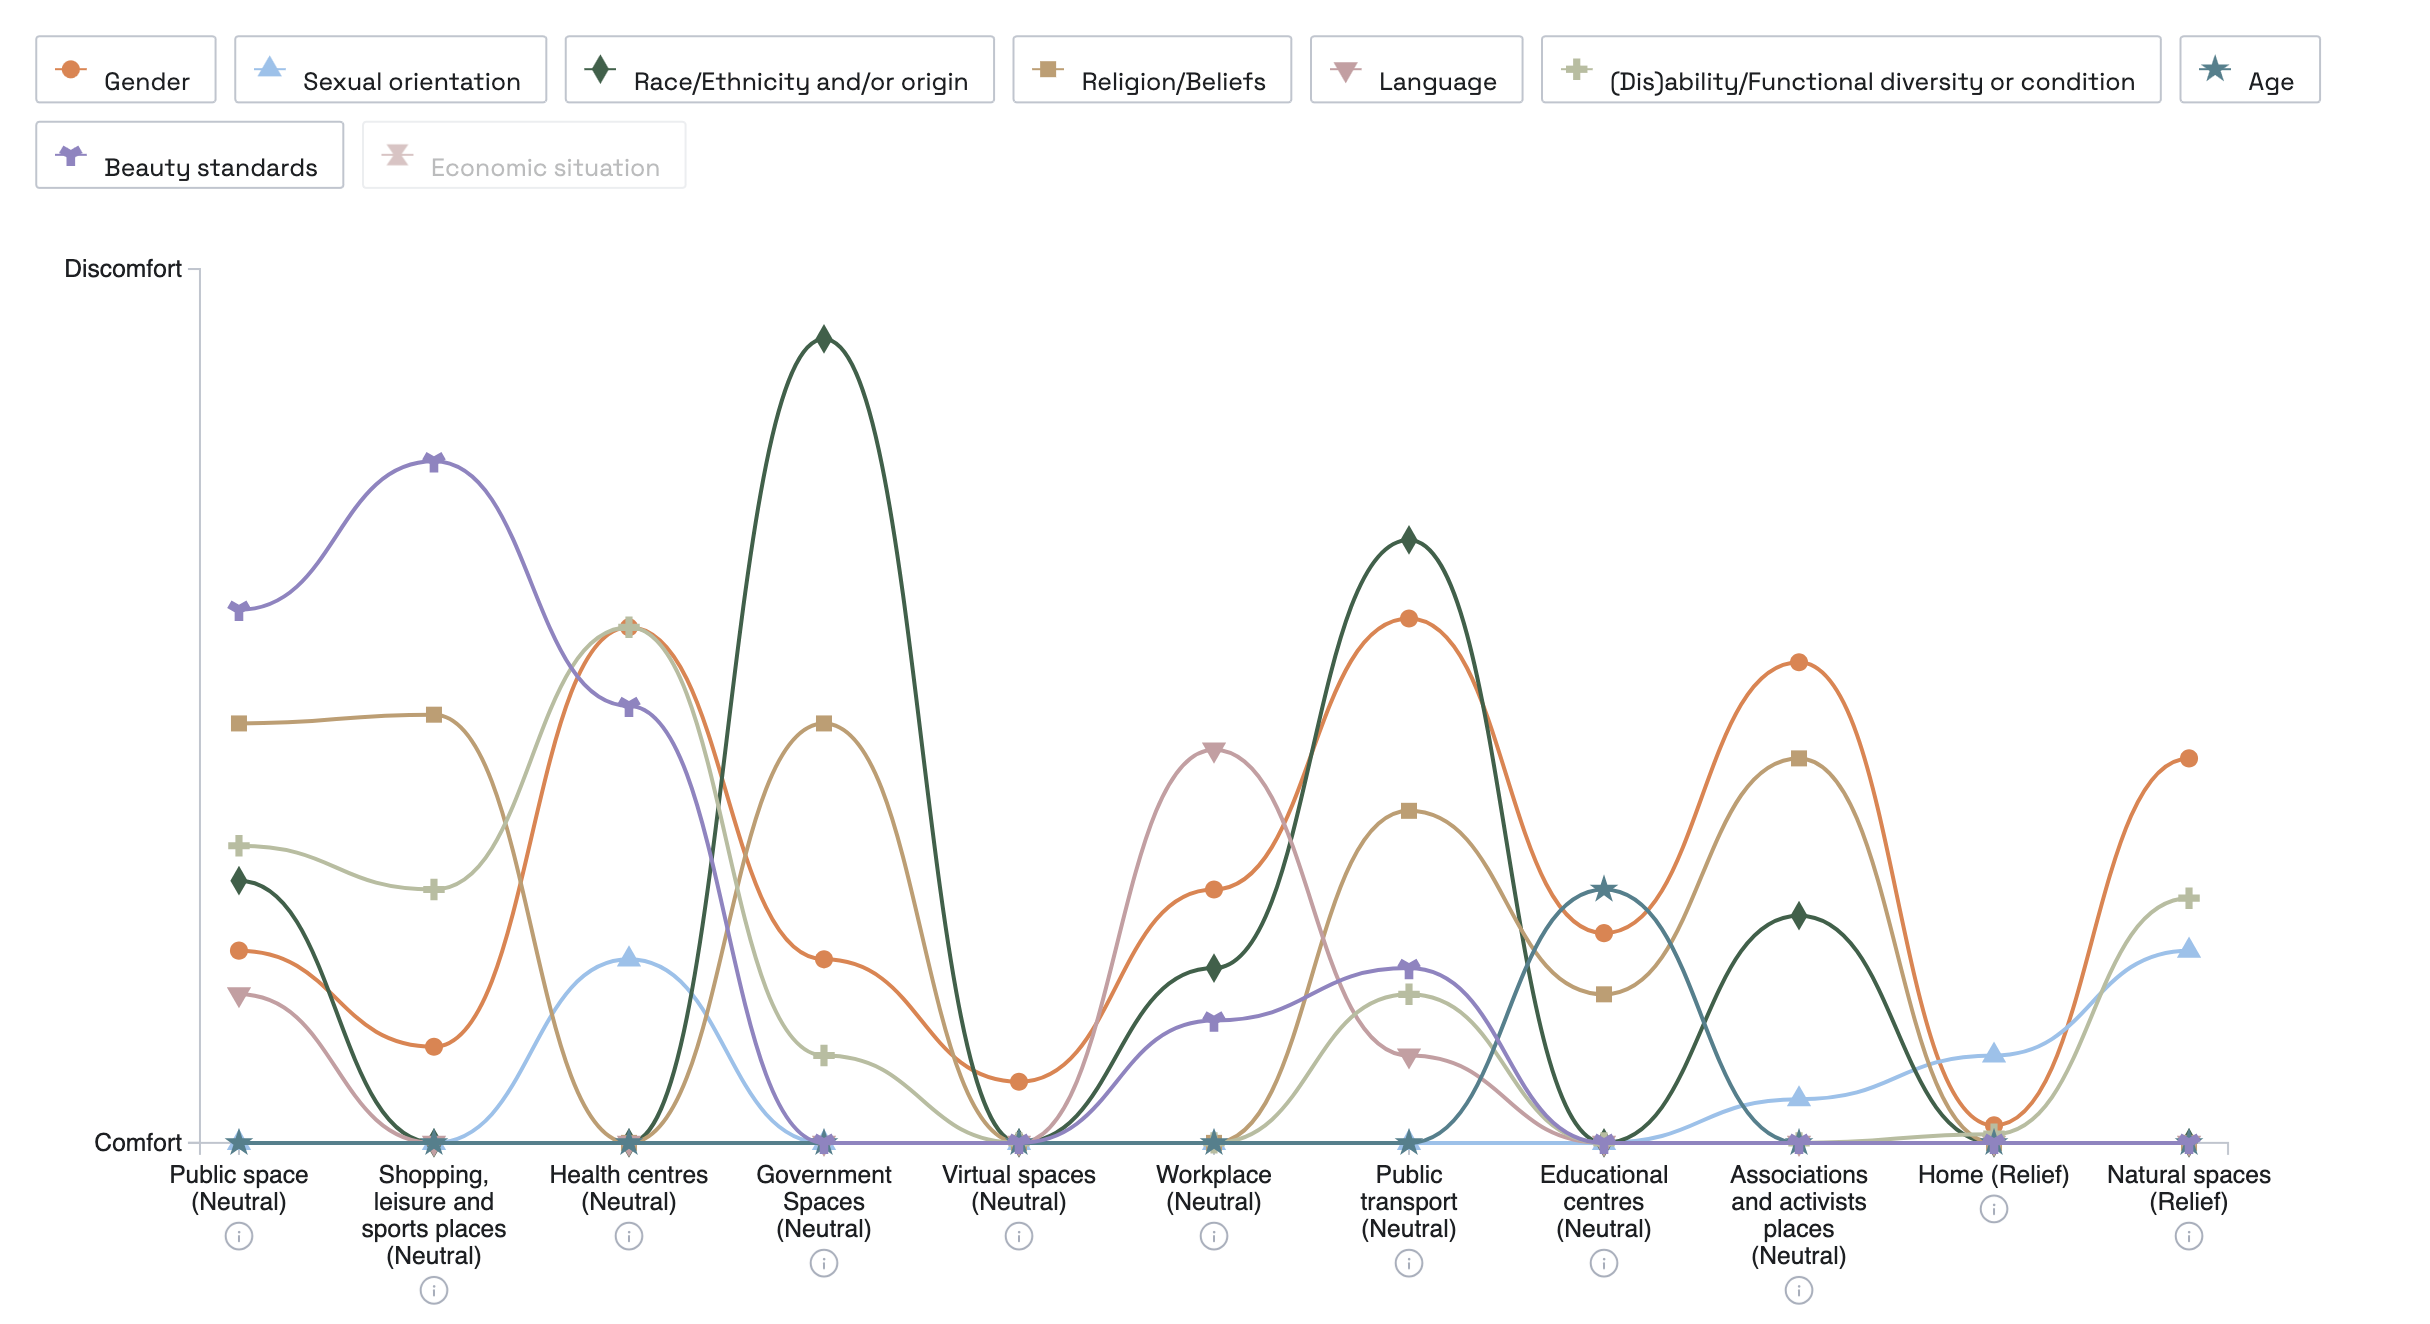
\includegraphics[width=\textwidth]{Arbeit/Bilder/reliefmap.png}
    \caption{Beispielhafte Ausgabe aus dem \gls{reliefmaps} Tool}
    \label{fig:relief_maps_plus_screenshot_1}
\end{figure}

Ein zentrales methodisches Merkmal von \gls{reliefmaps} ist der Versuch, die emotionale Wirkung sozialer Machtverhältnisse darstellbar zu machen -- ohne diese in eindimensionale Kausalbeziehungen zu überführen. Die Nutzer\genderstern innen bewerten ihre Erfahrungen explizit entlang einzelner \glspl{identitaetsachse}. Gleichzeitig zeigt sich hier eine zentrale methodologische Spannung: Die isolierte Betrachtung einzelner \glslink[noindex]{identitaetsachse}{Diskriminierungsachsen} widerspricht dem Grundgedanken einer \glslink[noindex]{intersektionalitaet}{intersektionaler} Analyse, der gerade auf die Verwobenheit und Gleichzeitigkeit verschiedener Machtverhältnisse verweist. Eine konsequente \glslink[noindex]{intersektionalitaet}{intersektionale} Operationalisierung bleibt damit methodisch herausfordernd.

Einige technische Merkmale von \gls{reliefmaps} sind auch im Hinblick auf die Entwicklung eigener Tools relevant. Die browserbasierte Anwendung erlaubt es Forschenden, eigenständig Projekte zu erstellen und auszuwerten. Allerdings ist der Zugang derzeit stark auf den katalanischen Kontext zugeschnitten: Verfügbare Sprachen sind aktuell nur Katalanisch, Spanisch und Englisch. Da der Quellcode nicht öffentlich zugänglich ist, bleiben Fragen zur Anpassbarkeit, Wiederverwendbarkeit und langfristigen Wartbarkeit offen. Aus methodischer Sicht stellt sich somit die Frage, inwiefern die Software übertragbar ist auf andere sprachliche, kulturelle und geografische Kontexte.

Trotz dieser Einschränkung eröffnet \gls{reliefmaps} wichtige Potenziale: Die bewusste Integration von Reflexivität, die aktive Beteiligung der Nutzer\genderstern innen an der Interpretation ihrer eigenen Erfahrungen sowie die Sichtbarmachung räumlich kontextualisierter Ungleichheiten markieren einen innovativen Zugang für \glslink[noindex]{intersektionalitaet}{intersektionale}, subjektzentrierte Geographien. Die methodische Fundierung des Tools beruht auf einem iterativen Validierungsprozess unter Einbezug feministischer, queerer und dekolonialer Perspektiven \parencite{luizdesouzaSpiralValidationProcess2025}.


\section{Offene Infrastruktur als Gegenentwurf}
\label{sec:offene_infrastruktur_als_gegenentwurf}

Ich verstehe die im Rahmen dieser Arbeit entwickelte App \gls[noindex]{intermind} (\gls{vgl} \cref{sec:entwicklung_app}) als offene, zugängliche und flexibel einsetzbare Plattform für \glsxtrshort[noindex]{ema} und \glsxtrshort[noindex]{gema}-Studien. Ich reagiere damit auf eine zentrale Leerstelle im bestehenden Tool-Ökosystem: Beide hier vorgestellten Anwendungen sind nicht quelloffen und dadurch weder vollständig nachvollziehbar noch unabhängig weiterentwickelbar. Dies betrifft nicht nur technische Details, sondern auch grundlegende Fragen der Datenverwendung, Kontrolle und Zugänglichkeit. Vor dem Hintergrund digitaler Souveränität (\gls[noindex]{vgl} \cref{sec:datafeminism}) stellt \gls[noindex]{intermind} daher bewusst nicht nur einen technischen, sondern auch einen forschungsethischen Gegenentwurf dar.

\gls[noindex]{intermind} versteht sich dabei nicht als methodische Neuerfindung, sondern als infrastrukturelle Ergänzung: Bestehende methodische Ansätze werden aufgegriffen und mit einem Fokus auf Offenheit und Modularität neu zusammengesetzt. Die Offenheit der Infrastruktur ist damit nicht nur technische Eigenschaft, sondern methodischer Anspruch.

Ziel des hier entwickelten Forschungsdesigns ist es, situiertes (Un\nobreakdash-)Wohlbefinden nicht nur als individuelle, sondern explizit als kontextuell-räumlich bedingte Erfahrungen wiederholt zu erfassen. Dieses Studiendesign bringt gegenüber querschnittbasierten Verfahren mehrere methodische Vorteile mit sich. Erstens reduziert die wiederholte intraindividuelle Erhebung Verzerrungen durch retrospektive Einschätzungen und erlaubt eine präzisere Erfassung situativer Schwankungen \parencite{randallDevelopmentTrialMobile2013}. Zweitens ermöglicht sie eine Kontrolle individueller Basisniveaus, was insbesondere für intersektionale Analysen relevant ist, die sowohl zwischen als auch innerhalb von Personen Differenzierungen vornehmen. Drittens erlaubt die Kombination von Echtzeitbefragung und intersektionaler Mehrebenenanalyse eine kontextsensitive Modellierung der Beziehungen zwischen affektivem Zustand und Umgebung im Sinne eines relationalen, ökologisch verstandenen Raumbegriffs.
